
Առանձին հետաքրքրություն են ներկայացնում այն դեկարտյան արտադրյալները, որոնք նաև հարթ գրաֆներ են: Հարթ դեկարտյան արտադրյալների միջակայքային ներկումներին անդրադառնալու համար կատարենք մի քանի նշանակումներ: $k$-չափանի ցանցը՝ $G(n_{1},n_{2},\ldots,n_{k})$, $n_{i}\in \mathbb{N}$, շղթաների դեկարտյան արտադրյալն է՝ $P_{n_{1}}\square P_{n_{2}}\square\cdots\square P_{n_{k}}$: Գլանը՝ $C(n_{1},n_{2})$, շղթայի և ցիկլի՝ $P_{n_{1}}\square C_{n_{2}}$, իսկ k-չափանի տոռը՝ $T(n_{1},n_{2},\ldots,n_{k})$, ցիկլերի դեկարտյան արտադրյալն է՝ $C_{n_{1}}\square C_{n_{2}}\square\cdots\square C_{n_{k}}$:

Բեհզադը և Մահմուդիանը \cite{BehzadMahmoodian1969} տվել են հարթ դեկարտյան արտադրյալների հետևյալ նկարագրությունը.

\begin{lemma}
\label{t2_behzad} $G \square H$ դեկարտյան արտադրյալը հարթ է այն և միայն դեպքում, եթե
\begin{enumerate}
    \item $G\square H \cong G(m,n)$,
    \item $G\square H \cong C(m,n)$ կամ
    \item $G \cong K_2$, իսկ $H$-ը արտաքին հարթ գրաֆ է:
\end{enumerate}
\end{lemma}

Այս պարագրաֆում հերթով կանդրադառնանք վերը նշված լեմմայում նկարագրված գրաֆների երեք դասերին: Հարթ դեկարտյան արտադրյալների միջակայքային ներկումների վերաբերյալ առաջին արդյունքը ստացել են Գիառոն և Կուբալը \cite{GiaroKubale1997}: Մասնավորապես, նրանք ցույց են տվել, որ $k$-չափանի ցանցերը, երկու չափանի տոռերը և այն գլանները, որոնց մեջ մասնակցող ցիկլը զույգ է, ունեն միջակայքային ներկում:

\begin{theorem}
\label{t2_Giaro_w} Եթե $G=G(n_{1},n_{2},\ldots,n_{k})$ կամ $G=C(m,2n)$, $m\in \mathbb{N}, n\geq 2$, կամ $G=T(2m,2n)$, $m,n\geq 2$, ապա $G\in \mathfrak{N}$ և $w(G)=\Delta(G)$:
\end{theorem}

Դիտարկենք ցանցերը: Հեշտ է տեսնել, որ $W\left(G(2,n)\right)=2n-1$ ցանկացած $n\in \mathbb{N}$-ի համար: Ստանանք ստորին գնահատական $W\left(G(m,n)\right)$-ի համար, երբ $m,n\geq 2$.

\begin{theorem}
\label{t2_grid_W} Ցանկացած $m,n\geq 2$ թվերի համար
\begin{center}
$W(G(m,n))\geq 2(m+n-3)$:
\end{center}
\end{theorem}
\begin{proof}[Ապացույց]Թեորեմն ապացուցելու համար կառուցենք $G(m,n)$ գրաֆի այնպիսի ներկում, որ կբավարարի նշված պայմաններին:

Դիցուք 
\begin{align*}
V(G(m,n))&=\left\{v_{j}^{(i)}\colon\,1\leq i\leq m,1\leq j\leq n\right\}\\
E(G(m,n))&=\bigcup_{i=1}^{m}E^{i}\cup \bigcup_{j=1}^{n}E_{j},
\end{align*}
որտեղ
\begin{center}
$E^{i}=\left\{v_{j}^{(i)}v_{j+1}^{(i)}\colon\,1\leq j\leq n-1
\right\}$ և $E_{j}=\left\{v_{j}^{(i)}v_{j}^{(i+1)}\colon\,1\leq
i\leq m-1\right\}$.
\end{center}

\begin{figure}[t!]
\centering
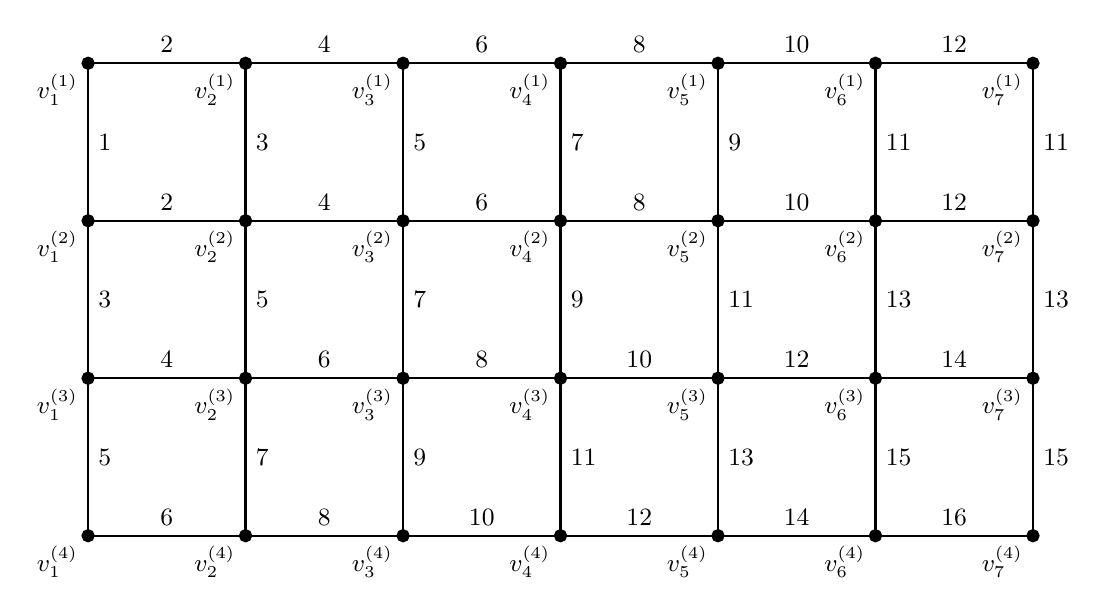
\begin{tikzpicture}[style=thick]
    \coordinate (V11) at (2cm,2cm);
    \coordinate (V12) at (4cm,2cm);
    \coordinate (V13) at (6cm,2cm);
    \coordinate (V14) at (8cm,2cm);
    \coordinate (V15) at (10cm,2cm);
    \coordinate (V16) at (12cm,2cm);
    \coordinate (V17) at (14cm,2cm);
    \coordinate (V21) at (2cm,4cm);
    \coordinate (V22) at (4cm,4cm);
    \coordinate (V23) at (6cm,4cm);
    \coordinate (V24) at (8cm,4cm);
    \coordinate (V25) at (10cm,4cm);
    \coordinate (V26) at (12cm,4cm);
    \coordinate (V27) at (14cm,4cm);
    \coordinate (V31) at (2cm,6cm);
    \coordinate (V32) at (4cm,6cm);
    \coordinate (V33) at (6cm,6cm);
    \coordinate (V34) at (8cm,6cm);
    \coordinate (V35) at (10cm,6cm);
    \coordinate (V36) at (12cm,6cm);
    \coordinate (V37) at (14cm,6cm);
    \coordinate (V41) at (2cm,8cm);
    \coordinate (V42) at (4cm,8cm);
    \coordinate (V43) at (6cm,8cm);
    \coordinate (V44) at (8cm,8cm);
    \coordinate (V45) at (10cm,8cm);
    \coordinate (V46) at (12cm,8cm);
    \coordinate (V47) at (14cm,8cm);
    
    \draw (V11) -- node[above] {$6$} (V12) -- node[above] {$8$} (V13) -- node[above] {$10$} (V14) -- node[above] {$12$} (V15) -- node[above] {$14$} (V16) -- node[above] {$16$} (V17);
    \draw (V21) -- node[above] {$4$} (V22) -- node[above] {$6$} (V23) -- node[above] {$8$} (V24) -- node[above] {$10$} (V25) -- node[above] {$12$} (V26) -- node[above] {$14$} (V27);
    \draw (V31) -- node[above] {$2$} (V32) -- node[above] {$4$} (V33) -- node[above] {$6$} (V34) -- node[above] {$8$} (V35) -- node[above] {$10$} (V36) -- node[above] {$12$} (V37);
    \draw (V41) -- node[above] {$2$} (V42) -- node[above] {$4$} (V43) -- node[above] {$6$} (V44) -- node[above] {$8$} (V45) -- node[above] {$10$} (V46) -- node[above] {$12$} (V47);
    
    \draw (V11) -- node[right] {$5$} (V21) -- node[right] {$3$} (V31) -- node[right] {$1$} (V41);
    \draw (V12) -- node[right] {$7$} (V22) -- node[right] {$5$} (V32) -- node[right] {$3$} (V42);
    \draw (V13) -- node[right] {$9$} (V23) -- node[right] {$7$} (V33) -- node[right] {$5$} (V43);
    \draw (V14) -- node[right] {$11$} (V24) -- node[right] {$9$} (V34) -- node[right] {$7$} (V44);
    \draw (V15) -- node[right] {$13$} (V25) -- node[right] {$11$} (V35) -- node[right] {$9$} (V45);
    \draw (V16) -- node[right] {$15$} (V26) -- node[right] {$13$} (V36) -- node[right] {$11$} (V46);
    \draw (V17) -- node[right] {$15$} (V27) -- node[right] {$13$} (V37) -- node[right] {$11$} (V47);
    
    \draw[fill=black] (V11) circle (2pt) node[below left]{$v_1^{(4)}$};
    \draw[fill=black] (V12) circle (2pt) node[below left]{$v_2^{(4)}$};
    \draw[fill=black] (V13) circle (2pt) node[below left]{$v_3^{(4)}$};
    \draw[fill=black] (V14) circle (2pt) node[below left]{$v_4^{(4)}$};
    \draw[fill=black] (V15) circle (2pt) node[below left]{$v_5^{(4)}$};
    \draw[fill=black] (V16) circle (2pt) node[below left]{$v_6^{(4)}$};
    \draw[fill=black] (V17) circle (2pt) node[below left]{$v_7^{(4)}$};
    \draw[fill=black] (V21) circle (2pt) node[below left]{$v_1^{(3)}$};
    \draw[fill=black] (V22) circle (2pt) node[below left]{$v_2^{(3)}$};
    \draw[fill=black] (V23) circle (2pt) node[below left]{$v_3^{(3)}$};
    \draw[fill=black] (V24) circle (2pt) node[below left]{$v_4^{(3)}$};
    \draw[fill=black] (V25) circle (2pt) node[below left]{$v_5^{(3)}$};
    \draw[fill=black] (V26) circle (2pt) node[below left]{$v_6^{(3)}$};
    \draw[fill=black] (V27) circle (2pt) node[below left]{$v_7^{(3)}$};
    \draw[fill=black] (V31) circle (2pt) node[below left]{$v_1^{(2)}$};
    \draw[fill=black] (V32) circle (2pt) node[below left]{$v_2^{(2)}$};
    \draw[fill=black] (V33) circle (2pt) node[below left]{$v_3^{(2)}$};
    \draw[fill=black] (V34) circle (2pt) node[below left]{$v_4^{(2)}$};
    \draw[fill=black] (V35) circle (2pt) node[below left]{$v_5^{(2)}$};
    \draw[fill=black] (V36) circle (2pt) node[below left]{$v_6^{(2)}$};
    \draw[fill=black] (V37) circle (2pt) node[below left]{$v_7^{(2)}$};
    \draw[fill=black] (V41) circle (2pt) node[below left]{$v_1^{(1)}$};
    \draw[fill=black] (V42) circle (2pt) node[below left]{$v_2^{(1)}$};
    \draw[fill=black] (V43) circle (2pt) node[below left]{$v_3^{(1)}$};
    \draw[fill=black] (V44) circle (2pt) node[below left]{$v_4^{(1)}$};
    \draw[fill=black] (V45) circle (2pt) node[below left]{$v_5^{(1)}$};
    \draw[fill=black] (V46) circle (2pt) node[below left]{$v_6^{(1)}$};
    \draw[fill=black] (V47) circle (2pt) node[below left]{$v_7^{(1)}$};
\end{tikzpicture}
\caption{$G(4,7)$ գրաֆի միջակայքային 16-ներկումը}
\label{grid}
\end{figure}

Սահմանենք $G(m,n)$-ի $\alpha$ կողային ներկում հետևյալ կերպ.
\begin{description}
\item[(1)] 
$\alpha\left(v_{j}^{(i)}v_{j}^{(i+1)}\right)=2(i+j)-3$ 
որտեղ $i=1,\ldots,m-1$, $j=1,\ldots,n-1$

\item[(2)] 
$\alpha\left(v_{n}^{(i)}v_{n}^{(i+1)}\right)=2(n+i)-5$
որտեղ $i=1,\ldots,m-1$

\item[(3)] 
$\alpha\left(v_{j}^{(1)}v_{j+1}^{(1)}\right)=2j$
որտեղ $j=1,\ldots,n-1$

\item[(4)] 
$\alpha\left(v_{j}^{(i)}v_{j+1}^{(i)}\right)=2(i+j)-4$
 որտեղ $i=2,\ldots,m$, $j=1,\ldots,n-1$
\end{description}

Հեշտ է տեսնել, որ $\alpha$-ն $G(m,n)$-ի միջակայքային $(2(m+n-3))$-ներկում է, երբ $m,n\geq 2$:
\end{proof}

Հարկ է նշել, որ Թեորեմ \ref{t2_grid_W}-ում ստացված գնահատականը հեռու չէ $W\left(G(m,n)\right)$-ի վերին գնահատականից: Քանի որ $G(m,n)$-ը երկկողմանի է, $2\leq \Delta\left(G(m,n)\right)\leq 4$ և
$\mathrm{diam}\left(G(m,n)\right)=m+n-2$, ապա Թեորեմ \ref{t1_upper_bipartite}-ից ստանում ենք $W\left(G(m,n)\right)\leq 3(m+n-2)+1$:

Թեորեմ \ref{t2_cartesian}-ից և Թեորեմ \ref{t2_grid_W}-ից ստանում ենք.

\begin{corollary}
\label{t2_n_grid_W} Եթե $n_{1}\geq\cdots \geq n_{2k}\geq 2$ $(k\in \mathbb{N})$, ապա
\begin{center}
$W(G(n_{1},n_{2},\ldots,n_{2k}))\geq 2\sum_{i=1}^{2k}n_{i}-6k$,
\end{center}
իսկ եթե $n_{1}\geq\cdots \geq n_{2k+1}\geq 2$ $(k\in \mathbb{N})$, ապա
\begin{center}
$W(G(n_{1},n_{2},\ldots,n_{2k+1}))\geq
2\sum_{i=1}^{2k}n_{i}+n_{2k+1}-6k-1$.
\end{center}
\end{corollary}

\bigskip

Այժմ դիտարկենք գլանները: Խչոյանը \cite{Kchoyan2010} ապացուցել է հետևյալը.

\begin{theorem}
\label{t2_Khchoyan} Ցանկացած $n\geq 3$ թվի համար
\begin{description}
\item[(1)] $C(2,n)\in \mathfrak{N}$,

\item[(2)] $w\left(C(2,n)\right)=3$,

\item[(3)] $W\left(C(2,n)\right)=n+2$,

\item[(4)] Եթե $w\left(C(2,n)\right)\leq t\leq W\left(C(2,n)\right)$, ապա $C(2,n)$-ը ունի միջակայքային $t$-ներկում:
\end{description}
\end{theorem}

Մեզ հաջողվել է ստանալ գլանների համար ավելի ընդհանուր արդյունք.

\begin{theorem}
\label{mytheorem16} Եթե $m\geq 3, n\in \mathbb{N}$, ապա $C(m,2n+1)\in \mathfrak{N}$ և
\begin{center}
$w\left(C(m,2n+1)\right)= \left\{
\begin{tabular}{ll}
$4$, & երբ $m$-ը զույգ է,\\
$6$, & երբ $m$-ը կենտ է:\\
\end{tabular}%
\right.$
\end{center}
\end{theorem}
\begin{proof}[Ապացույց] Դիցուք
\begin{align*}
    V(C(m,2n+1))&=\left\{v_{j}^{(i)}\colon\,1\leq i\leq m,1\leq j\leq 2n+1\right\}, \\
    E(C(m,2n+1))&=\bigcup_{i=1}^{m}{E}^{i}\cup \bigcup_{j=1}^{2n+1}{E}_{j},\text{ որտեղ}\\
    E^{i} &=\left\{v_{j}^{(i)}v_{j+1}^{(i)}\colon\,1\leq j\leq
    2n\right\}\cup \left\{v_{1}^{(i)}v_{2n+1}^{(i)}\right\},\\
    E_{j} &=\left\{v_{j}^{(i)}v_{j}^{(i+1)}\colon\,1\leq i\leq
m-1\right\}:
\end{align*}

Նախ ցույց տանք, որ եթե $m$-ը զույգ է, ապա $C(m,2n+1)$-ը ունի միջակայքային $4$-ներկում: Բոլոր $1\leq i\leq \frac{m}{2}$ թվերի համար սահմանենք $C(m,2n+1)$ գրաֆի $C^{i}$ ենթագրաֆը հետևյալ կերպ.
\begin{center}
$C^{i}=\left(V^{2i-1}\cup V^{2i},E^{2i-1}\cup E^{2i}\cup
\left\{v_{j}^{(2i-1)}v_{j}^{(2i)}\colon\,1\leq j\leq
2n+1\right\}\right)$:
\end{center}

$C^{i}$-ն իզոմորֆ է $C(2,2n+1)$ բոլոր $1\leq i\leq \frac{m}{2}$ թվերի համար. Թեորեմ \ref{t2_Khchoyan}-ի համաձայն, $C(2,2n+1)\in \mathfrak{N}$ և գոյություն ունի $C(2,2n+1)$ գրաֆի $\alpha$ միջակայքային $3$-ներկում: $C(m,2n+1)$-ի համար կայուցենք $\beta$ ներկումը:
Նախ $C^{i}$ ($1\leq i\leq\frac{m}{2}$) ենթագրաֆերի կողերը ներկենք համաձայն $\alpha$ ներկման: Այնուհետև $v_{j}^{(2i)}v_{j}^{(2i+1)}\in E_{j}$ կողերը ներկենք $4$ գույնով բոլոր $1\leq i\leq \frac{m}{2}-1, 1\leq j\leq 2n+1$ թվերի համար: Հեշտ է տեսնել, որ $\beta$-ն $C(m,2n+1)$-ի համար միջակայքային $4$-ներկում է: Այսպիսով, $C(m,2n+1)\in \mathfrak{N}$ և $w(C(m,2n+1))\leq 4$: Մյուս կողմից՝ $w(C(m,2n+1))\geq \Delta(C(m,2n+1))=4$, հետևաբար՝ $w(C(m,2n+1))=4$, երբ $m$-ը զույգ է:

\begin{figure}[b!]
\centering
\includegraphics[width=145mm]{figures/cylinders.jpg}
\caption{$C(m,2n+1)$ գրաֆի միջակայքային 6-ներկումը, երբ $n$-ը զույգ է (ձախից) և երբ $n$-ը կենտ է (աջից)}
\label{cylinders}
\end{figure}

Այժմ ենթադրենք $m$-ը կենտ է: Սկզբում ցույց տանք, որ $C(3,2n+1)$-ը ունի միջակայքային $6$-ներկում: Սահմանենք $C(3,2n+1)$-ի $\gamma$ կողային ներկումը հետևյալ կերպ.
\begin{description}
\item[(1)]
$\gamma\left(v_{1}^{(1)}v_{1}^{(2)}\right)=6$, $\gamma\left(v_{j}^{(1)}v_{j}^{(2)}\right)=4$, որտեղ $j=2,\ldots,2\left\lfloor\frac{n+1}{2}\right\rfloor$,
\item[(2)]
$\gamma\left(v_{2\left\lfloor\frac{n+1}{2}\right\rfloor+1}^{(1)}v_{2\left\lfloor\frac{n+1}{2}\right\rfloor+1}^{(2)}\right)=2$, $\gamma\left(v_{j}^{(1)}v_{j}^{(2)}\right)=3$, որտեղ  $j=2\left\lfloor\frac{n+1}{2}\right\rfloor+2,\ldots,2n+1$,
\item[(3)]
$\gamma\left(v_{1}^{(2)}v_{1}^{(3)}\right)=3$, $\gamma\left(v_{j}^{(2)}v_{j}^{(3)}\right)=2$, որտեղ $j=2,\ldots,2\left\lfloor\frac{n+1}{2}\right\rfloor$,
\item[(4)]
$\gamma\left(v_{j}^{(2)}v_{j}^{(3)}\right)=1$, որտեղ $j=2\left\lfloor\frac{n+1}{2}\right\rfloor+1,\ldots,2n+1$,
\item[(5)]
$\gamma\left(v_{2j-1}^{(1)}v_{2j}^{(1)}\right)=\gamma\left(v_{2j-1}^{(2)}v_{2j}^{(2)}\right)=5$
և
$\gamma\left(v_{2j}^{(1)}v_{2j+1}^{(1)}\right)=\gamma\left(v_{2j}^{(2)}v_{2j+1}^{(2)}\right)=3$,

որտեղ $j=1,\ldots,\left\lfloor\frac{n+1}{2}\right\rfloor,$

\item[(6)]
$\gamma\left(v_{2j-1}^{(1)}v_{2j}^{(1)}\right)=\gamma\left(v_{2j-1}^{(2)}v_{2j}^{(2)}\right)=4$
և
$\gamma\left(v_{1}^{(1)}v_{2n+1}^{(1)}\right)=\gamma\left(v_{1}^{(2)}v_{2n+1}^{(2)}\right)=4$,

 որտեղ $j=\left\lfloor\frac{n+1}{2}\right\rfloor+1,\ldots,n$,

\item[(7)]
$\gamma\left(v_{2j}^{(1)}v_{2j+1}^{(1)}\right)=\gamma\left(v_{2j}^{(2)}v_{2j+1}^{(2)}\right)=2$, որտեղ $j=\left\lfloor\frac{n+1}{2}\right\rfloor+1,\ldots,n$,

\item[(8)]
$\gamma\left(v_{2j-1}^{(3)}v_{2j}^{(3)}\right)=1$ և $\gamma\left(v_{2j}^{(3)}v_{2j+1}^{(3)}\right)=3$, որտեղ $j=1,\ldots,\left\lfloor\frac{n+1}{2}\right\rfloor$,

\item[(9)]
$\gamma\left(v_{2j-1}^{(3)}v_{2j}^{(3)}\right)=2$ և $\gamma\left(v_{1}^{(3)}v_{2n+1}^{(3)}\right)=2$, որտեղ $j=\left\lfloor\frac{n+1}{2}\right\rfloor+1,\ldots,n$,

\item[(10)]
$\gamma\left(v_{2j}^{(3)}v_{2j+1}^{(3)}\right)=3$, որտեղ $j=\left\lfloor\frac{n+1}{2}\right\rfloor+1,\ldots,n$:
\end{description}

Դժվար չէ տեսնել, որ $\gamma$-ն $C(3,2n+1)$-ի միջակայքային $6$-ներկում է, ընդ որում՝ $S(v_{j}^{(3)},\gamma)=[1,3]$ բոլոր $1\leq
j\leq 2n+1$ թվերի համար:

Այնուհետև կառուցենք $\phi$ ներկումը $C(m,2n+1)$ գրաֆի համար: Նախ ներկենք $C(m,2n+1)$-ի $C(3,2n+1)$ ենթագրաֆի կողերը՝ համաձայն $\gamma$ ներկման: Մնացած $C(m-3,2n+1)$ ենթագրաֆը ներկենք համաձայն $\beta$ ներկման: Վերջապես, $v_{j}^{(3)}v_{j}^{(4)}\in E_{j}$ ($1\leq j\leq 2n+1$) կողերը ներկենք $4$ գույնով: Հեշտ է տեսնել, որ $\phi$-ն $C(m,2n+1)$-ի միջակայքային $6$-ներկում է: Փաստորեն, $C(m,2n+1)\in \mathfrak{N}$ և $w(C(m,2n+1))\leq 6$.

Քանի որ կենտ $m$-երի դեպքում $G=C(m,2n+1)$ գրաֆը չունի կատարյալ զուգակցում, իսկ $\delta(G)=3$, $\Delta(G)=4$, ըստ Հետևանք \ref{c1_lower_nopm}-ի՝ $w(C(m,2n+1))\geq \max\left\{\Delta(G),2\delta(G)\right\} = 6$:
\end{proof}

Այսպիսով, մեզ հաջողվեց կառուցել միջակայքային ներկումներ ինչպես ցանցերի, այնպես էլ գլանների համար: Ունենալով այդ ներկումները և հաշվի առնելով Լեմմա \ref{t2_behzad}-ը, կարող ենք ձևակերպել հետևյալ պնդումը.

\begin{theorem}
\label{t2_planars} Եթե $G\square H$ դեկարտյան արտադրյալը հարթ է, ընդ որում 2 արտադրիչներն էլ ունեն առնվազն $3$ գագաթ, ապա $G\square H\in \mathfrak{N}$ և $w(G\square H)\leq 6$:
\end{theorem}

Գլանի ներկման համար անհրաժեշտ գույների առավելագույն քանակի համար Պետրոսյանը և Կարապետյանը \cite{PetrosyanKarapetyan2007} ստացել են ստորին գնահատական այն դեպքում, երբ գլանի բաղադրիչ ցիկլի երկարությունը զույգ է.
\begin{theorem}
\label{t2_cylinder_W_evencycle} Ցանկացած $m\in \mathbb{N}, n\geq 2$ թվերի համար
\begin{center}
$W(C(m,2n))\geq 3m+n-2$:
\end{center}
\end{theorem}

Մեզ հաջողվել ստանալ գնահատական այն դեպքում, երբ գլանի բաղադրիչ շղթայի երկարությունն է զույգ:
\begin{theorem}
\label{t2_cylinder_W_evenpath} Երբ $m\in\mathbb{N},n\geq 2$, 
\begin{center}
$W(C(2m,2n))\geq 4m+2n-2$,
\end{center}
իսկ երբ $m,n\in\mathbb{N}$,
\begin{center}
$W(C(2m,2n+1))\geq 4m+2n-1$:
\end{center}
\end{theorem}
\begin{proof}[Ապացույց] Թեորեմն ապացուցելու համար բավական է կառուցել համապատասխան պայմաններին բավարարող ներկումներ: Դիցուք, 
\begin{align*}
V(C(2m,2n))&=\left\{v_{j}^{(i)}\colon\,1\leq i\leq 2m,1\leq j\leq 2n\right\},\\
V(C(2m,2n+1))&=\left\{u_{j}^{(i)}\colon\,1\leq i\leq 2m,1\leq j\leq 2n+1\right\},\\
E(C(2m,2n))&=\bigcup_{i=1}^{2m}E^{i}\cup \bigcup_{j=1}^{2n}E_{j}, \\
E(C(2m,2n+1))&=\bigcup_{i=1}^{2m}\hat{E}^{i}\cup \bigcup_{j=1}^{2n+1}\hat{E}_{j},
\end{align*}
որտեղ 
\begin{align*}
E^{i}&=\left\{v_{j}^{(i)}v_{j+1}^{(i)}\colon\,1\leq j\leq
2n-1,\right\}\cup \left\{v_{1}^{(i)}v_{2n}^{(i)}\right\},
&E_{j}&=\left\{v_{j}^{(i)}v_{j}^{(i+1)}\colon\,1\leq i\leq
2m-1\right\},\\
\hat{E}^{i}&=\left\{u_{j}^{(i)}u_{j+1}^{(i)}\colon\,1\leq j\leq
2n,\right\}\cup \left\{u_{1}^{(i)}u_{2n+1}^{(i)}\right\},
&\hat{E}_{j}&=\left\{u_{j}^{(i)}u_{j}^{(i+1)}\colon\,1\leq i\leq
2m-1\right\}:
\end{align*}

Նախ կառուցենք $\alpha$ միջակայքային ներկումը $C(2m,2n)$ գրաֆի համար, որտեղ $m\in\mathbb{N},n\geq 2$:

\begin{description}
\item[(1)] 
$\alpha\left(v_{j}^{(2i-1)}v_{j+1}^{(2i-1)}\right)=\alpha\left(v_{j}^{(2i)}v_{j+1}^{(2i)}\right)=4i+2j-4$, որտեղ $i=1,\ldots,m$, $j=1,\ldots,n$,
\item[(2)] 
$\alpha\left(v_{j}^{(2i-1)}v_{j+1}^{(2i-1)}\right)=\alpha\left(v_{j}^{(2i)}v_{j+1}^{(2i)}\right)=4i-2j+4n-1$, որտեղ $i=1,\ldots,m$, $j=n+1,\ldots,2n-1$,
\item[(3)] 
$\alpha\left(v_{1}^{(2i-1)}v_{2n}^{(2i-1)}\right)=\alpha\left(v_{1}^{(2i)}v_{2n}^{(2i)}\right)=4i-1$, որտեղ $i=1,\ldots,m$,
\item[(4)] 
$\alpha\left(v_{j}^{(2i-1)}v_{j}^{(2i)}\right)=4i+2j-5$, որտեղ $i=1,\ldots,m$, $j=1,\ldots,n$,
\item[(5)] 
$\alpha\left(v_{j}^{(2i-1)}v_{j}^{(2i)}\right)=4i-2j+4n$, որտեղ $i=1,\ldots,m$, $j=n+1,\ldots,2n$,
\item[(6)] 
$\alpha\left(v_{j}^{(2i)}v_{j}^{(2i+1)}\right)=4i+2j-3$, որտեղ $i=1,\ldots,m-1$, $j=2,\ldots,n+1$,
\item[(7)] 
$\alpha\left(v_{j}^{(2i)}v_{j}^{(2i+1)}\right)=4i-2j+4n+2$, որտեղ $i=1,\ldots,m-1$, $j=n+2,\ldots,2n$,
\item[(8)] 
$\alpha\left(v_{1}^{(2i)}v_{1}^{(2i+1)}\right)=4i$, որտեղ $i=1,\ldots,m-1$:
\end{description}

Այժմ կառուցենք $\beta$ ներկումը $C(2m,2n+1)$ գրաֆի համար, որտեղ $m,n\in\mathbb{N}$:

\begin{description}
\item[(1)] 
$\beta\left(u_{j}^{(2i-1)}u_{j+1}^{(2i-1)}\right)=\beta\left(u_{j}^{(2i)}u_{j+1}^{(2i)}\right)=4i+2j-4$, որտեղ $i=1,\ldots,m$, $j=1,\ldots,n+1$,
\item[(2)] 
$\beta\left(u_{j}^{(2i-1)}u_{j+1}^{(2i-1)}\right)=\beta\left(u_{j}^{(2i)}u_{j+1}^{(2i)}\right)=4i-2j+4n+1$, որտեղ $i=1,\ldots,m$, $j=n+2,\ldots,2n$,
\item[(3)] 
$\beta\left(u_{1}^{(2i-1)}u_{2n+1}^{(2i-1)}\right)=\beta\left(u_{1}^{(2i)}u_{2n+1}^{(2i)}\right)=4i-1$, որտեղ $i=1,\ldots,m$,
\item[(4)] 
$\beta\left(u_{j}^{(2i-1)}u_{j}^{(2i)}\right)=4i+2j-5$, որտեղ $i=1,\ldots,m$, $j=1,\ldots,n+2$,
\item[(5)] 
$\beta\left(u_{j}^{(2i-1)}u_{j}^{(2i)}\right)=4i-2j+4n+2$, որտեղ $i=1,\ldots,m$, $j=n+3,\ldots,2n+1$,
\item[(6)] 
$\beta\left(u_{j}^{(2i)}u_{j}^{(2i+1)}\right)=4i+2j-3$, որտեղ $i=1,\ldots,m-1$, $j=2,\ldots,n+1$,
\item[(7)] 
$\beta\left(u_{j}^{(2i)}u_{j}^{(2i+1)}\right)=4i-2j+4n+4$, որտեղ $i=1,\ldots,m-1$, $j=n+2,\ldots,2n+1$,
\item[(8)] 
$\beta\left(u_{1}^{(2i)}u_{1}^{(2i+1)}\right)=4i$, որտեղ $i=1,\ldots,m-1$:
\end{description}

Դժվար չէ ստուգել, որ $\alpha$-ն $C(2m,2n)$-ի միջակայքային $(4m+2n-2)$-ներկում է, երբ $m\in\mathbb{N},n\geq 2$,
իսկ $\beta$-ն $C(2m,2n+1)$-ի միջակայքային $(4m+2n-1)$-ներկում է, երբ $m,n\in\mathbb{N}$:
\end{proof}

Նկատենք, որ երբ գլանի երկու բաղադրիչներն էլ ունեն զույգ թվով գագաթներ, \ref{t2_cylinder_W_evencycle} և \ref{t2_cylinder_W_evenpath} թեորեմները տալիս են տարբեր ստորին գնահատականներ $W\left(C(2m,2n)\right)$-ի համար: Երբ $n>2m$, Թեորեմ \ref{t2_cylinder_W_evenpath}-ի գնահատականը ավելի լավն է: Երբ $n=2m$, երկու թեորեմներն էլ տալիս են նույն գնահատականը: Իսկ երբ $n<2m$ ավելի լավն է Թեորեմ \ref{t2_cylinder_W_evencycle}-ի գնահատականը:

Թեորեմ \ref{t2_cylinder_W_evenpath}-ի ստորին գնահատականները հեռու չեն $W\left(C(2m,n)\right)$-ի համար հայտնի վերին գնահատականներից: Այսպես, քանի որ $C(2m,2n)$-ը երկկողմանի է, ընդ որում $3\leq \Delta\left(C(2m,2n)\right)\leq 4$ և $\mathrm{diam}\left(C(2m,2n)\right)=2m+n-1$, ապա Թեորեմ \ref{t1_upper_bipartite}-ից՝ $W\left(C(2m,2n)\right)\leq 3(2m+n-1)+1$: Նմանապես, քանի որ $3\leq \Delta\left(C(2m,2n+1)\right)\leq 4$ և $\mathrm{diam}\left(C(2m,2n+1)\right)=2m+n-1$, ապա Թեորեմ \ref{t1_upper}-ից՝ $W\left(C(2m,2n+1)\right)\leq 3(2m+n)+1$:


\subsubsection{Արտաքին հարթ գրաֆների ներկումներ}
\label{section_outerplanar}
Ինչպես տեսանք, $G\square H$ դեկարտյան արտադրյալը հարթ է նաև այն դեպքում, երբ $G=K_2$, իսկ $H$ գրաֆը արտաքին հարթ է: Մյուս կողմից, ըստ Թեորեմ \ref{t2_cartesian_gap}-ի, $G \square H$ արտադրյալը ունի միջակայքային ներկում այն և միայն դեպքում, երբ $H$-ը ունի միջակայքային մեկ անցքով ներկում: Այս պարագրաֆում կնկարագրենք արտաքին հարթ գրաֆների հատուկ տիպի ներկման կառուցման ալգորիթմ, որի շնորհիվ ցույց կտրվի, որ արտաքին հարթ գրաֆները բավարարում են Հիպոթեզ \ref{conj_def}-ին, իսկ եռանկյուն չպարունակող արտաքին գրաֆները նաև միջակայքային $1$-անցք-ներկելի են:

Ֆիորինին \cite{Fiorini1975} նկարագրել է բոլոր արտաքին հարթ գրաֆների քրոմատիկ դասը.
\begin{theorem}
Եթե $G$-ն արտաքին հարթ գրաֆ է, ապա $\chi'(G)=\Delta(G) + 1$ այն և միայն այն դեպքում, երբ $G$-ն կենտ ցիկլ է:
\end{theorem}

Թեորեմ \ref{t1_class1}-ից անմիջապես հետևում է, որ կենտ ցիկլերը միջակայքային ներկելի չեն: Սակայն գոյություն ունեն բազմաթիվ այլ արտաքին հարթ գրաֆներ, որոնց դեֆիցիտը դրական է: Օրինակ, Նկ. \ref{outerplanar-non-colorable}-ում պատկերված գրաֆը էյլերյան է, ունի կենտ թվով կողեր, և համաձայն Հետևանք \ref{c1_eulerian}-ի՝ չի կարող ունենալ միջակայքային ներկում: Մյուս կողմից, հեշտ է տեսնել, որ այդ գրաֆն ունի $1$ դեֆիցիտով ներկում:

\begin{figure}
  \begin{center}
  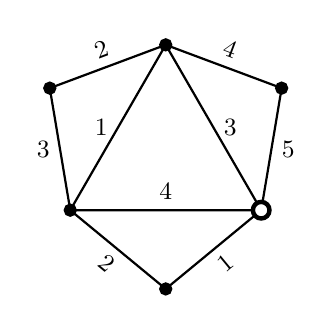
\begin{tikzpicture}[style=thick]
    \draw (90:1.4cm) -- node [right] {$3$}  
    (-30:1.4cm) -- node [sloped,above] {$4$} 
    (-150:1.4cm) -- node [left] {$1$} cycle;
    \draw (90:1.4cm) -- node [sloped,above] {$2$}  
    (150:1.7cm) -- node [left] {$3$}  
    (-150:1.4cm) -- node [sloped,below] {$2$}  
    (-90:1.7cm) -- node [sloped,below] {$1$}  
    (-30:1.4cm) -- node [right] {$5$} 
    (30:1.7cm) -- node [sloped,above] {$4$} cycle;
    
    \draw[fill=black] (90:1.4cm) circle (2pt);
    \draw[fill=white,style=ultra thick] (-30:1.4cm) circle (3pt);
    \draw[fill=black] (-150:1.4cm) circle (2pt);
    \draw[fill=black] (150:1.7cm) circle (2pt);
    \draw[fill=black] (-90:1.7cm) circle (2pt);
    \draw[fill=black] (30:1.7cm) circle (2pt);
  \end{tikzpicture}
  \end{center}
  \caption{Արտաքին հարթ տրիանգուլյացիա, որը միջակայքային ներկելի չէ: Պատկերված ներկման դեֆիցիտը $1$ է:}
  \label{outerplanar-non-colorable}
\end{figure}

Հայտնի է, որ արտաքին հարթ գրաֆների որոշ ենթադասեր միջակայքային ներկելի են: Արտաքին հարթ գրաֆը կոչվում է արտաքին հարթ տրիանգուլյացիա, եթե այն կարելի է պատկերել հարթության վրա այնպես, որ բոլոր սահմանափակ նիստերը լինեն եռանկյուն: Հարթության վրա պատկերված արտաքին հարթ գրաֆի եռանկյուն նիստը կոչվում է բաժանող եռանկյուն, եթե նրա կողմերից ոչ մեկը չի պատկանում անվերջ նիստին: Աքսենովիչը \cite{Axenovich2002} ապացուցել է հետևյալ թեորեմը.

\begin{theorem}
Եթե $G$-ն առնվազն չորս գագաթ պարունակող արտաքին հարթ տրիանգուլյացիա է և չունի բաժանող եռանկյուն, ապա այն միջակայքային ներկելի է:
\end{theorem}

Նկ. \ref{outerplanar-non-colorable}-ում պատկերված գրաֆը բաժանող եռանկյուն պարունակող արտաքին հարթ տրիանգուլյացիա է և չունի միջակայքային ներկում:

Հետագայում, Գիառոն և Կուբալեն \cite{GiaroKubale2004} նկարագրել են արտաքին հարթ գրաֆների միջակայքային ներկելի ևս մեկ ենթադաս.
\begin{theorem}
\label{t2_bipartite_outerplanar}
Եթե $G$-ն երկկողմանի արտաքին հարթ գրաֆ է, ապա այն միջակայքային ներկելի է:
\end{theorem}

Վերջապես, Պետրոսյանը \cite{Petrosyan2013Outerplanar} ստացել է հետևյալ արդյունքը.
\begin{theorem}
Եթե $G$-ն կապակցված ենթախորանարդ արտաքին հարթ գրաֆ է, բացի կենտ ցիկլից, ապա այն միջակայքային ներկելի է:
\end{theorem}

Այս պարագրաֆում մենք կդիտարկենք բոլոր արտաքին հարթ գրաֆների դեֆիցիտը և կընդհանրացնենք Թեորեմ  \ref{t2_bipartite_outerplanar}-ը:

$f_i(G)$-ով նշանակենք հարթության վրա պատկերված $G$ արտաքին հարթ գրաֆում $i$ կողեր ունեցող սահմանափակ նիստերի քանակը, որտեղ $i=3,4,\ldots,|V(G)|$:

\begin{lemma}
\label{outerplanar_basic_2connected}
Եթե $G$-ն համիլտոնյան արտաքին հարթ գրաֆ է, իսկ $w_0 \in V(G)$-ն այդ գրաֆի որևէ ֆիքսված գագաթ, ապա գոյություն ունի $G$-ի $\alpha$ ճիշտ կողային ներկում այնպիսին, որ.
\begin{itemize}
\item $def(w_0,\alpha)=0$,
\item $def(G,\alpha)=\sum\limits_{\substack{i\geq 3 \\ \text{կենտ }i}}{f_i(G)}$,
\item $gn(G,\alpha) \leq f_3(G) + \min\left\{1, \sum\limits_{\substack{i\geq 5 \\ \text{կենտ }i}}{f_{i}(G)}]\right\}$:
\end{itemize}
\end{lemma}
\begin{proof}[Ապացույց]
Այս լեմմայի ապացույցը ընդլայնում է \cite{DeWerraSolot1991}-ի Պնդում 3.1-ում և \cite{GiaroKubale2004}-ի Թեորեմ 2.3-ում մշակված մեթոդը:

Դիցուք $|V(G)|=n$ և $G$-ն պատկերված է հարթության վրա այնպես, որ բոլոր գագաթները պատկանում են անվերջ նիստին: $\alpha$ ներկումը կառուցելու ենք զուգահեռաբար ներկելով և նշելով $G$-ի կողերը: Կողերի նշումների ֆունկցիան նշանակենք $\lambda$-ով. $\lambda : E(G) \rightarrow \left\{\bm{l},\bm{u},\bm{m}\right\}$: Ալգորիթմի յուրաքանչյուր քայլում դիտարկվում է $G$-ի մեկ նիստ և, նիստին պատկանող կողերից մեկի նախապես որոշված գույնի և նշման հիման վրա միարժեքորեն որոշվում են մյուս կողերի գույները և նշումները: Նիստերի դիտարկման հերթականությունը որոշվում է ըստ $G$-ի $T$ թույլ երկակի գրաֆի: $T$-ի գագաթները համապատասխանում են $G$-ի սահմանափակ նիստերին և երկու գագաթներ միացած են կողով այն և միայն դեպքում, երբ համապատասխան նիստերը $G$-ում ունեն ընդհանուր կող: Հայտնի է, որ արտաքին հարթի թույլ երկակի գրաֆը անտառ է \cite{Harary1974}: Մեր դեպքում $G$-ն համիլտոնյան է, ուստի $2$-կապակցված է, հետևաբար թույլ երկակի գրաֆը ծառ է: Ստորև տրված է $\alpha$-ն և $\lambda$-ն կառուցող ալգորիթմի նկարագրությունը:

\begin{enumerate}
\item Պատկերենք $G$ գրաֆը հարթության վրա առանց խաչումների այնպես, որ բոլոր գագաթները պատկանեն անվերջ նիստին: Անվերջ նիստի կողերը կազմում են համիլտոնյան ցիկլ: Գրաֆի գագաթաները համակարալենք սկսած $w_0$-ից այդ ցիկլի երկայնքով ժամացույցի սլաքի ուղղությամբ. $w_0, w_1, \ldots, w_{n-1}$:
\item Կառուցենք $G$-ի $T$ թույլ երկակի գրաֆը:
\item Վերցնենք $G$-ի այն նիստը, որը պարունակում է $w_0w_{n-1}$ կողը: Դիցուք $t_0 \in V(T)$ գագաթը համապատասխանում է այդ նիստին: Նկատենք, որ այս նիստը միարժեք է որոշվում, քանի որ հակառակ դեպքում $w_0w_{n-1}$ կողը չէր պատկանի անվերջ նիստին: Դիցուք այդ նիստին պատկանող գագաթներն են $w_0=v_1,v_2,\ldots,v_r=w_{n-1}$ (ժամացույցի սլաքի ուղղությամբ):
\item Վերցնենք $\alpha(v_1v_r) = 1$ և $\lambda(v_1v_r)=\bm{u}$: \label{algo_set_first}
\item Լայնությամբ շրջանցենք $T$ ծառը՝ սկսելով $t_0$ գագաթից: Դիցուք $F$-ը $G$-ի այն նիստն է, որը համապատասխանում է տվյալ պահին դիտարկվող $t \in V(T)$ գագաթին: Ալգորիթմը երաշխավորում է, որ $F$-ի կողերից մեկը նախորդ քայլերից մեկում արդեն ներկվել և նշվել է: Դիցուք $V(F) = \left\{v_1,v_2,\ldots,v_r\right\}$ (ժամացույցի սլաքի ուղղությամբ), որտեղ $v_1v_r$-ը նախորդ քայլերից մեկում նշված կողն է և $\alpha(v_1v_r)=k$: Մնացած կողերի գույներն ու նշումները որոշվում են կախված $r$-ից և $\lambda(v_1v_r)$ նշումից (Նկ. \ref{outerplanar_figures}): \label{algo_traverse}
	\begin{enumerate}
    \item Եթե $\lambda(v_1v_r)=\bm{l}$, ապա ալգորիթմը երաշխավորում է, որ $\underline{S}(v_1, \alpha) = \underline{S}(v_r, \alpha) = k$, ուստի ներկումը կմնա ճիշտ, եթե նոր կողերին վերագրենք ավելի փոքր գույներ:
    	\begin{enumerate}
    	\item Եթե $r=3$, ապա վերցնենք $\alpha(v_1v_2)=k-1$, $\alpha(v_2v_3)=k-2$, $\lambda(v_1v_2)=\bm{m}$ և $\lambda(v_2v_3)=\bm{l}$: Նկատենք, որ $k-1$ գույնը բացակայում է $v_3$ գագաթի սպեկտրից և ալգորիթմի հաջորդ քայլերի ընթացքում ևս այդ գույնը չի օգտագործվի: \label{step3l}
        \item Եթե $r=2s$, $s\geq 2$, ապա $v_1v_2, v_2v_3, ..., v_{2s-1}v_{2s}$ կողերը ներկենք հերթականորեն $k-1$ և $k$ գույներով և նշենք հերթականորեն $\bm{l}$-ով և $\bm{u}$-ով: \label{step4l}
        \item Եթե $r=2s+1$, $s\geq 2$, ապա վերցնենք $\alpha(v_1v_2)=k-1$, $\alpha(v_2v_3)=k-2$, $\lambda(v_1v_2)=\bm{m}$, $\lambda(v_2v_3)=\bm{l}$, իսկ $v_3v_4, v_4v_5, ..., v_{2s}v_{2s+1}$ կողերը ներկենք հերթականորեն $k$ և $k-1$ գույներով և նշենք հերթականորեն $\bm{u}$-ով և $\bm{l}$-ով: Նկատենք, որ $v_3$ գագաթի սպեկտրից կբացակայի $k-1$ գույնը:\label{step5l}
    	\end{enumerate}
    
    \item Եթե $\lambda(v_1v_r)=\bm{u}$, ապա ալգորիթմը երաշխավորում է, որ $\overline{S}(v_1, \alpha) = \overline{S}(v_r, \alpha) = k$, ուստի ներկումը կմնա ճիշտ, եթե նոր կողերի վրա օգտագործենք ավելի մեծ գույներ:
    	\begin{enumerate}
    	\item Եթե $r=3$, ապա վերցնենք $\alpha(v_1v_2)=k+1$, $\alpha(v_2v_3)=k+2$, $\lambda(v_1v_2)=\bm{m}$ և $\lambda(v_2v_3)=\bm{u}$: Նկատենք, որ $v_3$ գագաթի սպեկտրից կբացակայի $k+1$ գույնը: \label{step3u}
        \item Եթե $r=2s$, $s\geq 2$, ապա $v_1v_2, v_2v_3, ..., v_{2s-1}v_{2s}$ կողերը ներկենք հերթականորեն $k-1$ և $k$ գույներով և նշենք հերթականորեն $\bm{u}$-ով և $\bm{l}$-ով: \label{step4u}
        \item Եթե $r=2s+1$, $s\geq 2$, ապա վերցնենք $\alpha(v_1v_2)=k+1$, $\alpha(v_2v_3)=k+2$, $\lambda(v_1v_2)=\bm{m}$, $\lambda(v_2v_3)=\bm{u}$, իսկ $v_3v_4, v_4v_5, ..., v_{2s}v_{2s+1}$ կողերը ներկենք հերթականորեն $k$ և $k+1$ գույներով և նշենք հերթականորեն $\bm{l}$-ով և $\bm{u}$-ով: Նկատենք, որ $v_3$ գագաթի սպեկտրում չի մասնակցի $k+1$ գույնը:\label{step5u}
    	\end{enumerate}
    \item Եթե $\lambda(v_1v_r)=\bm{m}$, ապա ալգորիթմը երաշխատվորում է, որ կա՛մ $\overline{S}(v_1,\alpha) = \underline{S}(v_r,\alpha) = k$, կա՛մ $\underline{S}(v_1,\alpha) = \overline{S}(v_r,\alpha) = k$:
    	\begin{enumerate}
    	\item Եթե $\underline{S}(v_1,\alpha) = \overline{S}(v_r,\alpha) = k$, ապա $F$ նիստի գագաթները վերահամարակալենք ժամացույցի սլաքի հակառակ ուղղությամբ՝ այսպիսով երաշխավորելով, որ $\overline{S}(v_1,\alpha) = \underline{S}(v_r,\alpha) = k$: \label{stepmrename}
        \item Եթե $r=3$, ապա վերցնենք $\alpha(v_1v_2)=k+1$, $\alpha(v_2v_3)=k-1$, $\lambda(v_1v_2)=\bm{u}$ և $\lambda(v_2v_3)=\bm{l}$: Նկատենք, որ $v_2$ գագաթի սպեկտրում չի մասնակցի $k$ գույնը: \label{step3m}
        \item Եթե $r=2s$, $s\geq 2$, ապա վերցնենք $\alpha(v_1v_2)=k+1$, $\alpha{v_2v_3} = k$, $\lambda(v_1v_2)=\bm{u}$ և $\lambda(v_2v_3)=\bm{m}$: Այնուհետև $v_3v_4, v_4v_5, ..., v_{2s-1}v_{2s}$ կողերը ներկենք հերթականորեն $k-1$ և $k$ գույներով և նշենք հերթականորեն $\bm{u}$-ով և $\bm{l}$-ով: \label{step4m}
        \item Եթե $r=2s+1$, $s\geq 2$, ապա վերցնենք $\alpha(v_1v_2)=k+1$, $\lambda(v_1v_2)=\bm{u}$, իսկ $v_2v_3, v_3v_4, ..., v_{2s}v_{2s+1}$ կողերը ներկենք հերթականորեն $k-1$ և $k$ գույներով և նշենք հերթականորեն $\bm{l}$-ով և $\bm{u}$-ով:\label{step5m}
    	\end{enumerate}
	\end{enumerate}
    \item Եթե $\min_{e \in E(G)}\alpha(e) = c_0 \ne 1$, ապա բոլոր կողերի գույները շեղենք համաձայն $\alpha(e) = \alpha(e) - c_0 + 1$ ($e \in E(G)$), բանաձևի:
\end{enumerate}

\begin{figure}
\tikzset{font=\fontsize{9pt}{12}}
\begin{tabular}{|m{.024\textwidth}| m{.22\textwidth} | m{.287\textwidth} | m{.334\textwidth}|}
\hline
 & $r=3$ & $r=2s$, $s\geq 2$ & $r=2s+1$, $s\geq 2$ \\
\hline
$\bm{l}$ & 
  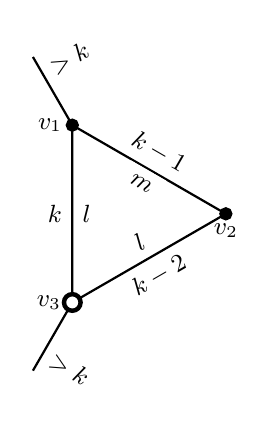
\begin{tikzpicture}[style=thick]
    \draw (120:1.3cm) -- node [sloped,above] {$k-1$} node [sloped,below, fill=white] {$\bm{m}$} (0:1.3cm) -- node [sloped,above] {$\bm{l}$} node [sloped,below] {$k-2$} (240:1.3cm);
    
    \draw (120:2.3cm) -- node [right,sloped,near start,rotate=90] {$>k$}
    (120:1.3cm) -- node [left] {$k$} node [right] {$\bm{l}$} 
    (-120:1.3cm) -- node [right,sloped,near end,rotate=-90] {$>k$}
    (-120:2.3cm);
    
    \draw[fill=black] (120:1.3cm) circle (2pt) node [left] {$v_1$};
    \draw[fill=black] (0:1.3cm) circle (2pt) node [below] {$v_2$};
    \draw[fill=white,style=ultra thick] (-120:1.3cm) circle (3pt) node [left] {$v_3$};
  \end{tikzpicture} & 
  
  
  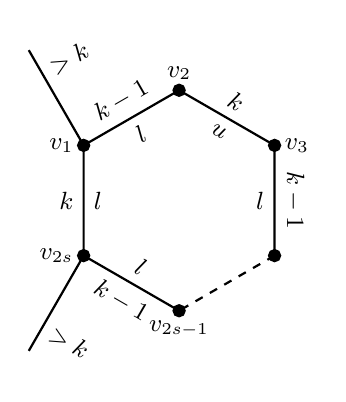
\begin{tikzpicture}[style=thick]
    \draw (150:1.4cm) -- node [sloped,above] {$k-1$} node [sloped,below] {$\bm{l}$} 
    (90:1.4cm) -- node [sloped,above] {$k$} node [sloped,below] {$\bm{u}$} 
    (30:1.4cm) -- node [sloped,above] {$k-1$} node [left] {$\bm{l}$} 
    (-30:1.4cm);
    \draw (-30:1.4cm) -- 
    (-90:1.4cm) [dashed];
    \draw (-90:1.4cm) -- node [sloped,below] {$k-1$} node [sloped,above] {$\bm{l}$} 
    (-150:1.4cm);
    
    \draw (135:2.7cm) -- node [right,sloped,near start,rotate=90] {$>k$}
    (150:1.4cm) -- node [left] {$k$} node [right] {$\bm{l}$} 
    (-150:1.4cm) -- node [right,sloped,near end,rotate=-90] {$>k$}
    (-135:2.7cm);
    
    \draw[fill=black] (150:1.4cm) circle (2pt) node [left] {$v_1$};
    \draw[fill=black] (90:1.4cm) circle (2pt) node [above] {$v_2$};
    \draw[fill=black] (30:1.4cm) circle (2pt) node [right] {$v_3$};
    \draw[fill=black] (-30:1.4cm) circle (2pt);
    \draw[fill=black] (-90:1.4cm) circle (2pt) node [below] {$v_{2s-1}$};
    \draw[fill=black] (-150:1.4cm) circle (2pt) node [left] {$v_{2s}$};
  \end{tikzpicture} & 
  
  
  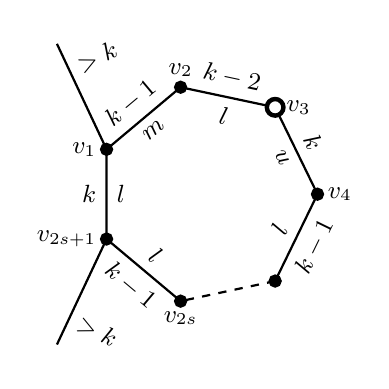
\begin{tikzpicture}[style=thick]
    \draw (156:1.4cm) -- node [sloped,above] {$k-1$} node [sloped,below] {$\bm{m}$} 
    (104:1.4cm) -- node [sloped,above] {$k-2$} node [sloped,below] {$\bm{l}$} 
    (52:1.4cm) -- node [sloped,above] {$k$} node [sloped,below] {$\bm{u}$} 
    (0:1.4cm) -- node [sloped,below] {$k-1$} node [sloped,above] {$\bm{l}$} 
    (-52:1.4cm);
    \draw (-52:1.4cm) -- 
    (-104:1.4cm) [dashed];
    \draw (-104:1.4cm) -- node [sloped,above] {$\bm{l}$} node [sloped,below] {$k-1$} 
    (-156:1.4cm);
    
    \draw (135:2.7cm) -- node [right,sloped,near start,rotate=90] {$>k$}
    (156:1.4cm) -- node [left] {$k$} node [right] {$\bm{l}$} 
    (-156:1.4cm) -- node [right,sloped,near end,rotate=-90] {$>k$}
    (-135:2.7cm);
    
    \draw[fill=black] (156:1.4cm) circle (2pt) node [left] {$v_1$};
    \draw[fill=black] (104:1.4cm) circle (2pt) node [above] {$v_2$};
    \draw[fill=white,style=ultra thick] (52:1.4cm) circle (3pt) node [right] {$v_3$};
    \draw[fill=black] (0:1.4cm) circle (2pt) node [right] {$v_4$};
    \draw[fill=black] (-52:1.4cm) circle (2pt);
    \draw[fill=black] (-104:1.4cm) circle (2pt) node [below] {$v_{2s}$};
    \draw[fill=black] (-156:1.4cm) circle (2pt) node [left] {$v_{2s+1}$};
  \end{tikzpicture} \\
\hline


$\bm{u}$ & 
  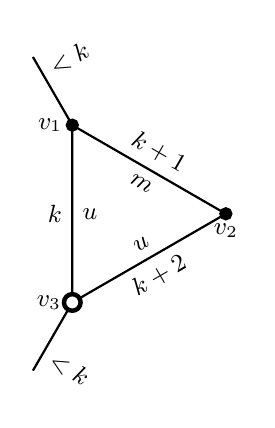
\begin{tikzpicture}[style=thick]
    \draw (120:1.3cm) -- node [sloped,above] {$k+1$} node [sloped,below] {$\bm{m}$} (0:1.3cm) -- node [sloped,above] {$\bm{u}$} node [sloped,below] {$k+2$} (240:1.3cm);
    
    \draw (120:2.3cm) -- node [right,sloped,near start,rotate=90] {$<k$}
    (120:1.3cm) -- node [left] {$k$} node [right] {$\bm{u}$} 
    (-120:1.3cm) -- node [right,sloped,near end,rotate=-90] {$<k$}
    (-120:2.3cm);
    
    \draw[fill=black] (120:1.3cm) circle (2pt) node [left] {$v_1$};
    \draw[fill=black] (0:1.3cm) circle (2pt) node [below] {$v_2$};
    \draw[fill=white,style=ultra thick] (-120:1.3cm) circle (3pt) node [left] {$v_3$};
  \end{tikzpicture} & 
  
  
  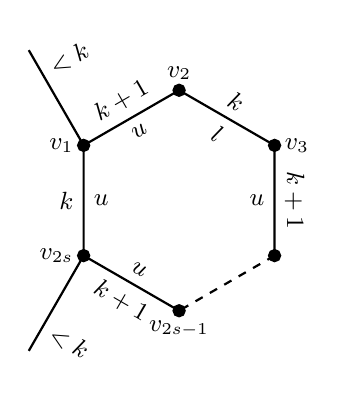
\begin{tikzpicture}[style=thick]
    \draw (150:1.4cm) -- node [sloped,above] {$k+1$} node [sloped,below] {$\bm{u}$} 
    (90:1.4cm) -- node [sloped,above] {$k$} node [sloped,below] {$\bm{l}$} 
    (30:1.4cm) -- node [sloped,above] {$k+1$} node [left] {$\bm{u}$} 
    (-30:1.4cm);
    \draw (-30:1.4cm) -- 
    (-90:1.4cm) [dashed];
    \draw (-90:1.4cm) -- node [sloped,below] {$k+1$} node [sloped,above] {$\bm{u}$} 
    (-150:1.4cm);
    
    \draw (135:2.7cm) -- node [right,sloped,near start,rotate=90] {$<k$}
    (150:1.4cm) -- node [left] {$k$} node [right] {$\bm{u}$} 
    (-150:1.4cm) -- node [right,sloped,near end,rotate=-90] {$<k$}
    (-135:2.7cm);
   
    \draw[fill=black] (150:1.4cm) circle (2pt) node [left] {$v_1$};
    \draw[fill=black] (90:1.4cm) circle (2pt) node [above] {$v_2$};
    \draw[fill=black] (30:1.4cm) circle (2pt) node [right] {$v_3$};
    \draw[fill=black] (-30:1.4cm) circle (2pt);
    \draw[fill=black] (-90:1.4cm) circle (2pt) node [below] {$v_{2s-1}$};
    \draw[fill=black] (-150:1.4cm) circle (2pt) node [left] {$v_{2s}$};
  \end{tikzpicture} & 
  
  
  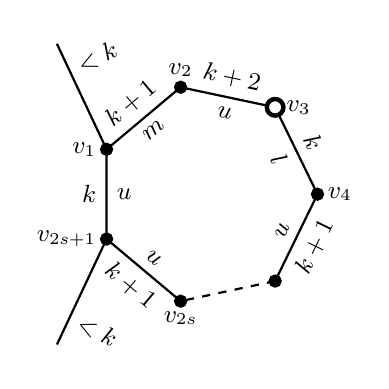
\begin{tikzpicture}[style=thick]
    \draw (156:1.4cm) -- node [sloped,above] {$k+1$} node [sloped,below] {$\bm{m}$} 
    (104:1.4cm) -- node [sloped,above] {$k+2$} node [sloped,below] {$\bm{u}$} 
    (52:1.4cm) -- node [sloped,above] {$k$} node [sloped,below] {$\bm{l}$} 
    (0:1.4cm) -- node [sloped,below] {$k+1$} node [sloped,above] {$\bm{u}$} 
    (-52:1.4cm);
    \draw (-52:1.4cm) -- 
    (-104:1.4cm) [dashed];
    \draw (-104:1.4cm) -- node [sloped,below] {$k+1$} node [sloped,above] {$\bm{u}$} 
    (-156:1.4cm);
    
    \draw (135:2.7cm) -- node [right,sloped,near start,rotate=90] {$<k$}
    (156:1.4cm) -- node [left] {$k$} node [right] {$\bm{u}$} 
    (-156:1.4cm) -- node [right,sloped,near end,rotate=-90] {$<k$}
    (-135:2.7cm);
    
    \draw[fill=black] (156:1.4cm) circle (2pt) node [left] {$v_1$};
    \draw[fill=black] (104:1.4cm) circle (2pt) node [above] {$v_2$};
    \draw[fill=white,style=ultra thick] (52:1.4cm) circle (3pt) node [right] {$v_3$};
    \draw[fill=black] (0:1.4cm) circle (2pt) node [right] {$v_4$};
    \draw[fill=black] (-52:1.4cm) circle (2pt);
    \draw[fill=black] (-104:1.4cm) circle (2pt) node [below] {$v_{2s}$};
    \draw[fill=black] (-156:1.4cm) circle (2pt) node [left] {$v_{2s+1}$};
  \end{tikzpicture} \\
\hline


$\bm{m}$ & 
  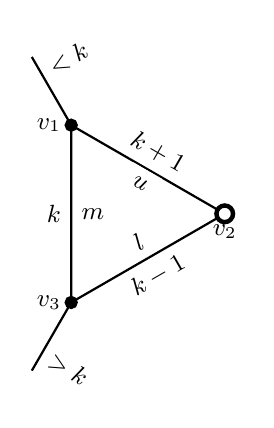
\begin{tikzpicture}[style=thick]
    \draw (120:1.3cm) -- node [sloped,above] {$k+1$} node [sloped,below, fill=white] {$\bm{u}$} (0:1.3cm) -- node [sloped,above] {$\bm{l}$} node [sloped,below] {$k-1$} (240:1.3cm);
    
    \draw (120:2.3cm) -- node [right,sloped,near start,rotate=90] {$<k$}
    (120:1.3cm) -- node [left] {$k$} node [right] {$\bm{m}$} 
    (-120:1.3cm) -- node [right,sloped,near end,rotate=-90] {$>k$}
    (-120:2.3cm);
    
    \draw[fill=black] (120:1.3cm) circle (2pt) node [left] {$v_1$};
    \draw[fill=white,style=ultra thick] (0:1.3cm) circle (3pt) node [below] {$v_2$};
    \draw[fill=black] (-120:1.3cm) circle (2pt) node [left] {$v_3$};
  \end{tikzpicture} & 
  
  
  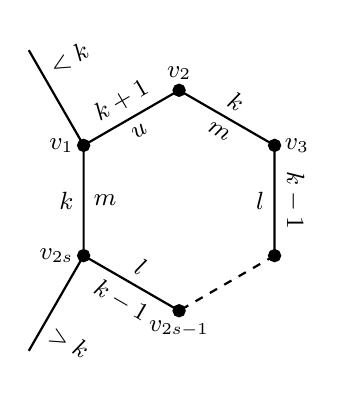
\begin{tikzpicture}[style=thick]
    \draw (150:1.4cm) -- node [sloped,above] {$k+1$} node [sloped,below] {$\bm{u}$} 
    (90:1.4cm) -- node [sloped,above] {$k$} node [sloped,below] {$\bm{m}$} 
    (30:1.4cm) -- node [sloped,above] {$k-1$} node [left] {$\bm{l}$} 
    (-30:1.4cm);
    \draw (-30:1.4cm) -- 
    (-90:1.4cm) [dashed];
    \draw (-90:1.4cm) -- node [sloped,above] {$\bm{l}$} node [sloped,below] {$k-1$} 
    (-150:1.4cm);
    
    \draw (135:2.7cm) -- node [right,sloped,near start,rotate=90] {$<k$}
    (150:1.4cm) -- node [left] {$k$} node [right] {$\bm{m}$} 
    (-150:1.4cm) -- node [right,sloped,near end,rotate=-90] {$>k$}
    (-135:2.7cm);
    
    \draw[fill=black] (150:1.4cm) circle (2pt) node [left] {$v_1$};
    \draw[fill=black] (90:1.4cm) circle (2pt) node [above] {$v_2$};
    \draw[fill=black] (30:1.4cm) circle (2pt) node [right] {$v_3$};
    \draw[fill=black] (-30:1.4cm) circle (2pt);
    \draw[fill=black] (-90:1.4cm) circle (2pt) node [below] {$v_{2s-1}$};
    \draw[fill=black] (-150:1.4cm) circle (2pt) node [left] {$v_{2s}$};
  \end{tikzpicture} & 
  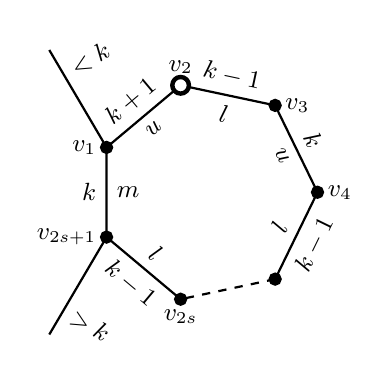
\begin{tikzpicture}[style=thick]
    \draw (156:1.4cm) -- node [sloped,above] {$k+1$} node [sloped,below] {$\bm{u}$} 
    (104:1.4cm) -- node [sloped,above] {$k-1$} node [sloped,below] {$\bm{l}$} 
    (52:1.4cm) -- node [sloped,above] {$k$} node [sloped,below] {$\bm{u}$} 
    (0:1.4cm) -- node [sloped,below] {$k-1$} node [sloped,above] {$\bm{l}$} 
    (-52:1.4cm);
    \draw (-52:1.4cm) -- 
    (-104:1.4cm) [dashed];
    \draw (-104:1.4cm) -- node [sloped,above] {$\bm{l}$} node [sloped,below] {$k-1$} 
    (-156:1.4cm);
    
    \draw (138:2.7cm) -- node [right,sloped,near start,rotate=90] {$<k$}
    (156:1.4cm) -- node [left] {$k$} node [right] {$\bm{m}$} 
    (-156:1.4cm) -- node [right,sloped,near end,rotate=-90] {$>k$}
    (-138:2.7cm);
    
    \draw[fill=black] (156:1.4cm) circle (2pt) node [left] {$v_1$};
    \draw[fill=white,style=ultra thick] (104:1.4cm) circle (3pt) node [above] {$v_2$};
    \draw[fill=black] (52:1.4cm) circle (2pt) node [right] {$v_3$};
    \draw[fill=black] (0:1.4cm) circle (2pt) node [right] {$v_4$};
    \draw[fill=black] (-52:1.4cm) circle (2pt);
    \draw[fill=black] (-104:1.4cm) circle (2pt) node [below] {$v_{2s}$};
    \draw[fill=black] (-156:1.4cm) circle (2pt) node [left] {$v_{2s+1}$};
  \end{tikzpicture} \\
\hline
\end{tabular}

\tikzset{font=\small}
\caption{Լեմմա \ref{outerplanar_basic}-ում նկարագրված ալգորիթմի Քայլ \ref{algo_traverse}-ի նկարագրությունը: Աղյուսակի տողերը համապատասխանում են $v_1v_r$ կողի նշմանը: Սյուները համապատասխանում են հերթական $F$ նիստի կողերի քանակին: Օղակներով նշված գագաթները (ի տարբերություն շրջաններով նշվածների) ցույց են տալիս, որ ալգորիթմի տվյալ քայլի արդյունքում այդ գագաթի սպեկտրներում չօգտագործված գույների քանակը (դեֆիցիտը) կավելանա մեկով:}
\label{outerplanar_figures}
\end{figure}

Ապացույցն ավարտելու համար անհրաժեշտ է ստուգել լեմմայի երեք պնդումները: Նախ, նկատենք, որ ալգորիթմը կենտ թվով կողեր ունեցող յուրաքանչյուր նիստի գագաթներից մեկի սպեկտրում ավելացնում է ճիշտ մեկ չօգտագործված գույն (\ref{step3l}, \ref{step3u}, \ref{step3m}, \ref{step5l}, \ref{step5u} և \ref{step5m} քայլերում): Ավելին, ալգորիթմը չի ավելացնում նոր չօգտագործված գույն զույգ թվով կողեր ունեցող նիստի գագաթներում (\ref{step4l}, \ref{step4u}, \ref{step4m} քայլերում): Այստեղից հետևում է, որ բոլոր գագաթների սպեկտրներում բացակայող գույների քանակը հավասար է կենտ կողեր ունեցող նիստերի քանակին. $def(G,\alpha) = \sum_{i\geq 3,\text{կենտ }i}{f_i(G)}$:

Այնուհետև, կարևոր է նկատել, որ որևէ գագաթի դեֆիցիտը մեկից մեծ կլինի միայն այն դեպքում, երբ ալգորիթմը այդ գագաթում բացակայող գույն ավելացնի այդ գագաթը պարունակող մեկից ավելի իրարից տարբեր նիստեր դիտարկելու ընթացքում: Երբ $r \geq 5$ (\ref{step5l}, \ref{step5u} և \ref{step5m} քայլեր) կամ երբ $r=3$ և $\lambda(v_1v_3)=\bm{m}$ (Քայլ \ref{step3m}), բացակայող գույնը ավելացվում է այնպիսի գագաթներում, որոնք նախորդ քայլերում չեն դիտարկվել: Ուստի գագաթի դեֆիցիտը կարող է դառնալ մեկից ավել միայն \ref{step3l} և \ref{step3u} քայլերի դեպքում ($r=3$, և $\lambda(v_1v_r)=\bm{l}$ կամ $\lambda(v_1v_r)=\bm{u}$): Այսպիսով, կամայական գագաթի դեֆիցիտը չի կարող լինել $G$-ում եռանկյունների քանակին գումարած մեկ թվից, այն դեպքում, երբ այն պատկանում է նաև ավելի մեծ կենտ ցիկլի: Հետևաբար, $gn(G,\alpha) = \max_{v\in V(G)}{\left\{def(v,\alpha)\right\}} \leq f_3(G) + \min\left\{1, \sum_{i\geq 5,\text{կենտ }i}{f_i(G)}\right\}$: Այստեղ հավասարությունը դառնում է հասանելի, երբ $G$-ն հովհար գրաֆ է:

Վերջապես պետք է ցույց տալ, որ $def(w_0, \alpha)=0$: Ենթադրենք այս գագաթը պատկանում է թվով $k \geq 1$ տարբեր նիստերի: Այս նիստերը դիտարկվում են $T$ ծառի լայնական շրջանցմամբ որոշվող հերթականությամբ: \ref{algo_set_first} քայլից հետո յուրաքանչյուր անգամ, երբ դիտարկվում է այս $k$ նիստերից մեկը, $w_0$ գագաթը պատկանում է արդեն ներկված կողին և նշանակվում է $v_1$-ով: Միակ բացառությունը \ref{stepmrename} քայլն է, երբ $\lambda(v_1v_r)= \bf{m}$ և $w_0$ գագաթը կարող է նշանակված լինել $v_r$-ով: Նկատենք, որ անկախ դիտարկվող նիստի $r$ երկարությունից և $\lambda(v_1v_r)$ նշումից, $v_1$ գագաթում նոր բացակայող գույն չի ավելանում:
\end{proof}

Հաջորդ թեորեմը ապացուցելու համար անհրաժեշտ է բլոկների և միակցման կետերի ծառի գաղափարը: Բլոկը մաքսիմալ $2$-կապակցված ենթագրաֆն է: Միակցման կետը այնպիսի գագաթ է, որը հանելու դեպքում գրաֆի կապակցվածության բաղադրիչների քանակը ավելանում է: Տրված $G$ գրաֆի համար $B$-ով նշանակենք իր բլոկների բազմությունը, իսկ $C$-ով՝ իր միակցման կետերի բազմությունը: Նկատենք, որ կամայական միակցման կետ պատկանում է առնվազն երկու բլոկի: Կառուցենք $bc(G)$ գրաֆը հետևյալ կերպ. $V(bc(G)) = B \cup C$, իսկ $b \in B$ և $c \in C$ գագաթները միացվում են կողով այն և միայն այն դեպքում, երբ $G$ գրաֆում $c$ գագաթը պատկանում է $b$ բլոկին: Հայտնի է, որ $bc(G)$-ն ծառ է \cite{Harary1969}: $bc(G)$-ն կոչվում է $G$-ի բլոկների և միակցման կետերի գրաֆ:

\begin{theorem}
\label{outerplanar_basic}
Եթե $G$-ն արտաքին հարթ գրաֆ է, ապա 
\begin{center}
$def(G) \leq \sum\limits_{\substack{i\geq 3 \\ \text{կենտ }i}}{f_i(G)}$ և $gn(G) \leq f_3(G) + \min\left\{1, \sum\limits_{\substack{i\geq 5 \\ \text{կենտ }i}}{f_{i}(G)}\right\}$:
\end{center}
\end{theorem}
\begin{proof}[Ապացույց]
Դիցուք $bc(G)$-ն $G$-ի բլոկների և միակցման կետերի գրաֆն է: $G$-ի բլոկները նշանակենք $B_1, B_2, \ldots, B_m$, $m\geq 1$, իսկ միակցման կետերը՝ $c_1, \ldots c_n$, $n \geq 0$: Բլոկները կա՛մ իզոմորֆ են $K_2$-ին, կա՛մ համիլտոնյան արտաքին հարթ գրաֆներ են: $G$-ի $\beta$ ներկումը կառուցենք բլոկների ներկումների հիման վրա: Սկսենք $B_1$ գագաթին համապատասխանող բլոկից: Եթե $B_1$-ը իզոմորֆ է $K_2$-ին, ապա իր միակ կողը ներկենք $1$ գույնով: Եթե այն համիլտոնյան արտաքին հարթ գրաֆ է, ապա վերցնենք $\beta(e) = \alpha_1(e)$, բոլոր $e \in E(B_1)$ կողերի համար, որտեղ $\alpha_1$-ը $B_1$-ի ներկումն է ըստ Լեմմա \ref{outerplanar_basic_2connected}-ի:

Այնուհետև, կատարենք $bc(G)$ ծառի լայնական շրջանցում: Ենթադրենք հասել ենք $B_i \in V(bc(G))$ բլոկին: $bc(G)$ ծառում այս բլոկի ծնողը որևէ $c_k$ միակցման կետ է, որի ծնողը իր հերթին որևէ այլ $B_j$ բլոկ է, որն ալգորիթմի նախորդ քայլերում արդեն ներկվել է: Ենթադրենք այդ պահին $\overline{S}(c_k, \beta) = t$: Կառուցենք $B_i$ բլոկի $\alpha_i$ ներկումը: Եթե $B_i$-ն իզոմորֆ է $K_2$-ին, ապա նրա միակ կողը ներկենք $1$ գույնով: Հակառակ դեպքում, որպես $\alpha_i$ վերցնենք $B_i$ բլոկի ներկումը համաձայն Լեմմա \ref{outerplanar_basic_2connected}-ի՝ վերցնելով $w_0 = c_k$, որպեսզի երաշխավորվի, որ $def(c_k,\alpha_i) = 0$: $G$-ի համապատասխան կողերը ներկենք հետևյալ բանաձևով. $\beta(e) = \alpha_i(e) + t$, բոլոր $e \in E(B_i)$ կողերի համար: Այսպես կերաշխավորվի, որ $B_i$ բլոկը ներկելուց հետո $def(c_k, \beta)$ դեֆիցիտը կմնա հավասար $def(c_k, \alpha_j)$-ին:

Հեշտ է տեսնել, որ
\begin{align*}
def(G,\beta) &= \sum\limits_{k}{def(G,\alpha_k)} =  \sum\limits_{k}{ \sum\limits_{\substack{i\geq 3 \\ \text{կենտ }i}}{f_i(B_k)} } = \sum\limits_{\substack{i\geq 3 \\ \text{կենտ }i}}{f_i(G)},\\
gn(G,\beta) &= \max\limits_{k}{gn(G,\alpha_k)} \leq \max\limits_{k}{\left\{f_3(B_k) + \min\left\{1, \sum\limits_{\substack{i\geq 5 \\ \text{կենտ }i}}{f_{i}(B_k)}\right\}\right\}} \leq \\
&\leq f_3(G) + \min\left\{1, \sum\limits_{\substack{i\geq 5 \\ \text{կենտ }i}}{f_{i}(G)}\right\}:
\end{align*}
\end{proof}

\begin{corollary}
Եթե $G$-ն երկկողմանի արտաքին հարթ գրաֆ է, ապա այն միջակայքային ներկելի է:
\end{corollary}

\begin{corollary}
Եթե $G$-ն եռանկյուն չպարունակող արտաքին հարթ գրաֆ է, ապա այն միջակայքային $1$-անցք-ներկելի է:
\end{corollary}

\begin{corollary}
\label{c2_outerlanar_def}
Եթե $G$-ն արտաքին հարթ գրաֆ է, ապա 
\begin{center}
$def(G) \leq \frac{|V(G)|-2}{og(G)-2}$,
\end{center}
որտեղ $og(G)$-ն $G$-ի կարճագույն կենտ ցիկլի երկարությունն է:
\end{corollary}
\begin{proof}[Ապացույց]
Կամայական համիլտոնյան արտաքին հարթ գրաֆ կարելի է կառուցել սկսելով $K_2$-ից և իտերատիվ կերպով ավելացնելով սահմանափակ նիստեր: Յուրաքանչյուր ավելացված սահմանափակ նիստ, որն ունի $m$ կող, ավելացնում է ճիշտ $m-2$ գագաթներ: Այսպիսով, երբ $G$-ն համիլտոնյան է, $|V(G)| = 2 + \sum\limits_{i\geq 3}f_i(G)(i-2)$: Ընդհանուր դեպքում, երբ $B_1, \ldots, B_k$, $k \geq 1$, հանդիսանում են $G$-ի բլոկները, ունենք, որ 
\begin{align*}
|V(G)| &\geq 1 + \sum\limits_{j=1}^{k}{\left(|V(B_j)|-1\right)} \geq 1 + \sum\limits_{j=1}^{k}{\left(2 + \sum\limits_{i\geq 3}f_i(B_j)(i-2) - 1\right)} \\
&\geq 2 + \sum\limits_{i\geq 3}f_i(G)(i-2) \geq 2 + \sum\limits_{\substack{i\geq 3\\\text{կենտ }i}}{f_i(G)(i-2)} \geq 2 + \sum\limits_{\substack{i\geq 3\\\text{կենտ }i}}{f_i(G)(og(G)-2)}:
\end{align*}
Վերջին անհավասարությունը տեղի ունի, քանի որ կամայական կենտ կողեր ունեցող նիստ ունի առնվազն $og(G)$ կող: Հաշվի առնելով Թեորեմ \ref{outerplanar_basic}-ը, ստանում ենք, որ
$def(G) \leq \sum\limits_{\substack{i\geq 3\\\text{կենտ }i}}{f_i(G)} \leq \frac{|V(G)| - 2}{og(G)-2}$:
\end{proof}

Գիառոն, Կուբալը և Մալաֆիյսկին ցույց են տվել, որ գոյություն ունի գրաֆների $\left\{G_n\right\}$ հաջորդականություն այնպես, որ $\lim_{n \rightarrow \infty}{\frac{def(G_n)}{|V(G_n)|}} = 1$ \cite{GiaroKubaleMalafiejski1999}: Մյուս կողմից՝ հայտնի չեն գրաֆներ, որոնց դեֆիցիտը գագաթների թվից մեծ է: Գրաֆների դեֆիցիտի վերաբերյալ կարևորագույն բաց խնդիրներից է հետևյալ հիպոթեզը.
\begin{hypothesis}
\label{conj_def}
Ցանկացած $G$ գրաֆի համար $def(G) \leq |V(G)|$:
\end{hypothesis}

Հիպոթեզը ակնհայտորեն ճիշտ է միջակայքային $1$-անցք-ներկելի գրաֆների համար, այդ թվում՝ համասեռ գրաֆների համար: Մյուս կողմից, հայտնի է, որ կամայական $h$ թվի համար գոյություն ունի գրաֆ, որը միջակայքային $h$-անցք-ներկելի չէ \cite{PetrosyanKhachatrianCID2013}: Հետևանք \ref{c2_outerlanar_def}-ից հետևում է, որ արտաքին հարթ գրաֆները բավարարում են Հիպոթեզ \ref{conj_def}-ին:
